\documentclass[a4paper]{article}

\usepackage{pgfplots}

\pgfplotsset{compat=1.5}

\begin{document}

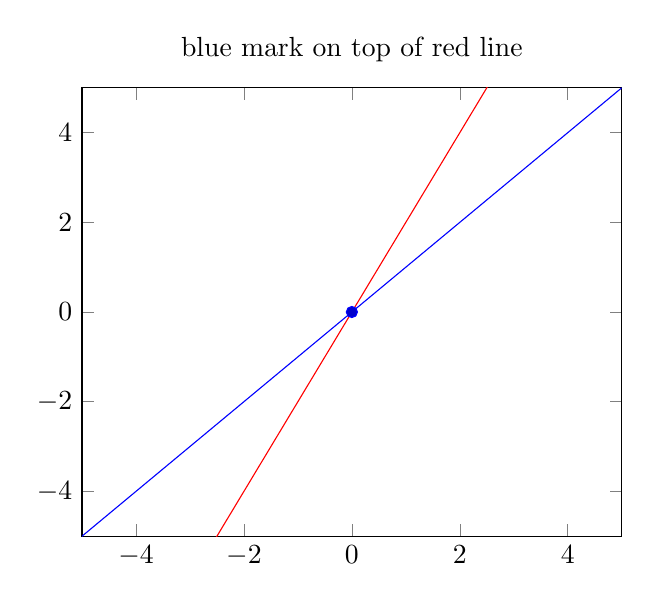
\begin{tikzpicture}
	\begin{axis}[xmin=-5,xmax=5,ymin=-5,ymax=5,domain=-10:10,title=blue mark on top of red line]
	\addplot+[samples=3] {x};	
	\addplot+[samples=2] {2*x};	
	\end{axis}
\end{tikzpicture}

\begin{tikzpicture}
	\begin{axis}[clip=plots individually,xmin=-5,xmax=5,ymin=-5,ymax=5,domain=-10:10, title=blue mark below red line]
	\addplot+[samples=3] {x};	
	\addplot+[samples=2] {2*x};	
	\end{axis}
\end{tikzpicture}

\begin{tikzpicture}
	\begin{axis}[clip=plots individually,use layers,mark layer=unclipped axis foreground,xmin=-5,xmax=5,ymin=-5,ymax=5,domain=-10:10, title=blue mark above red line (mark layer)]
	\addplot+[samples=3] {x};	
	\addplot+[samples=2] {2*x};	
	\end{axis}
\end{tikzpicture}
\end{document}

